\begin{frame}
\frametitle{Image Registration}
\begin{columns}[c]
\column{0.7\textwidth}
\begin{itemize}
\item Image registration finds shortest distance between images.
\item Often formulated to minimise the sum of two terms:
\begin{itemize}
\item Distance between the image intensities.
\item Distance of the deformation from the identity.
\end{itemize}
\item The sum of these gives a distance.
\end{itemize}
\column{0.3\textwidth}
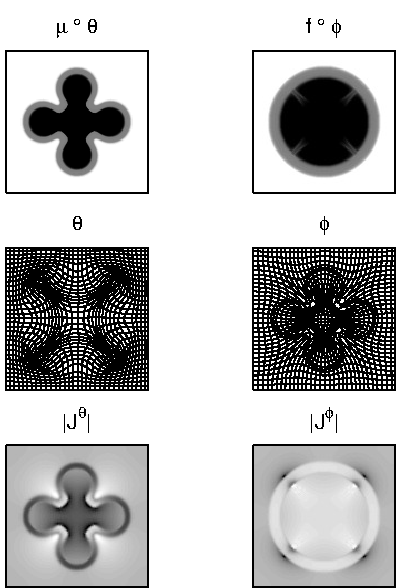
\includegraphics[width=\textwidth]{shoot2d}
\end{columns}
\end{frame}

%%%%%%%%%%%%%%%%%%%%%%%%%%%%%%%%%%%%%%%%%%%%%%%%%%%%%%%%%%%%%%%
\begin{frame}
\frametitle{LDDMM}
\emph{Large Deformation Diffeomorphic Metric Mapping} is an image registration algorithm that minimises the following:
\begin{eqnarray*}
\mathcal{E}  =   \frac{1}{2} \int_{t=0}^1  || {\bf L} {\bf v}_t ||^2 dt +
                 \frac{1}{2\sigma^2} || f - \mu\left({\boldsymbol\varphi}_1^{-1}\right)||^2\\
\text{  where } {\boldsymbol\varphi}_0 = \mathrm{id} \text{, } \frac{d{\boldsymbol\varphi}}{dt} = {\bf v}_t\left({\boldsymbol\varphi}_t\right)
\end{eqnarray*}
First term is a squared deformation distance measure.\par
Second term is the squared difference between images.\par
The objective is to estimate a series of velocity fields (${\bf v}_t$).\par
%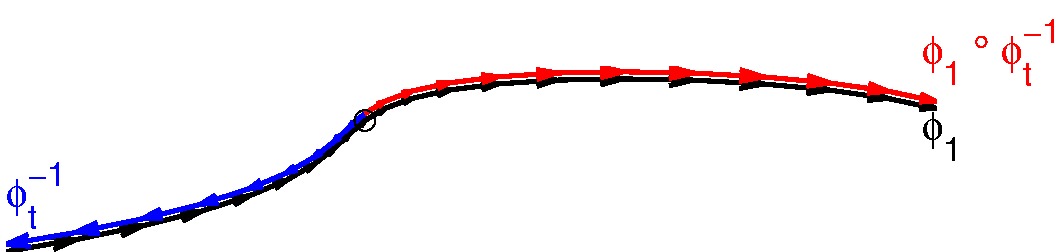
\includegraphics[width=\textwidth]{trajectory}
%These may be conceptualised as
%\begin{eqnarray*}
%\frac{d {\boldsymbol\varphi}}{d t} = {\bf v}_t ({\boldsymbol\varphi})
%\end{eqnarray*}
\vspace{.25cm}
\begin{tiny}
Beg, MF, Miller, MI, Trouv{\'e}, A \& Younes, L. \emph{Computing large deformation metric mappings via geodesic flows of diffeomorphisms}. International Journal of Computer Vision 61(2):139--157 (2005).\par
\end{tiny}
\end{frame}

%%%%%%%%%%%%%%%%%%%%%%%%%%%%%%%%%%%%%%%%%%%%%%%%%%%%%%%%%%%%%%%

%\begin{frame}
%\frametitle{Different ways of measuring distances}
%\begin{columns}[c]
%\column{.2\textwidth}
%\begin{center}
%Two simulated images\par
%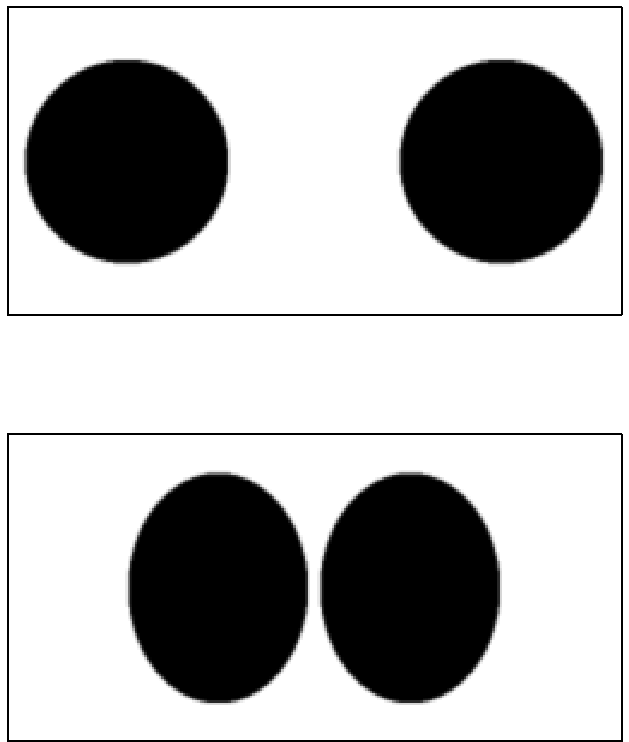
\includegraphics[width=\textwidth]{figure2Di}
%\end{center}
%\column{.8\textwidth}
%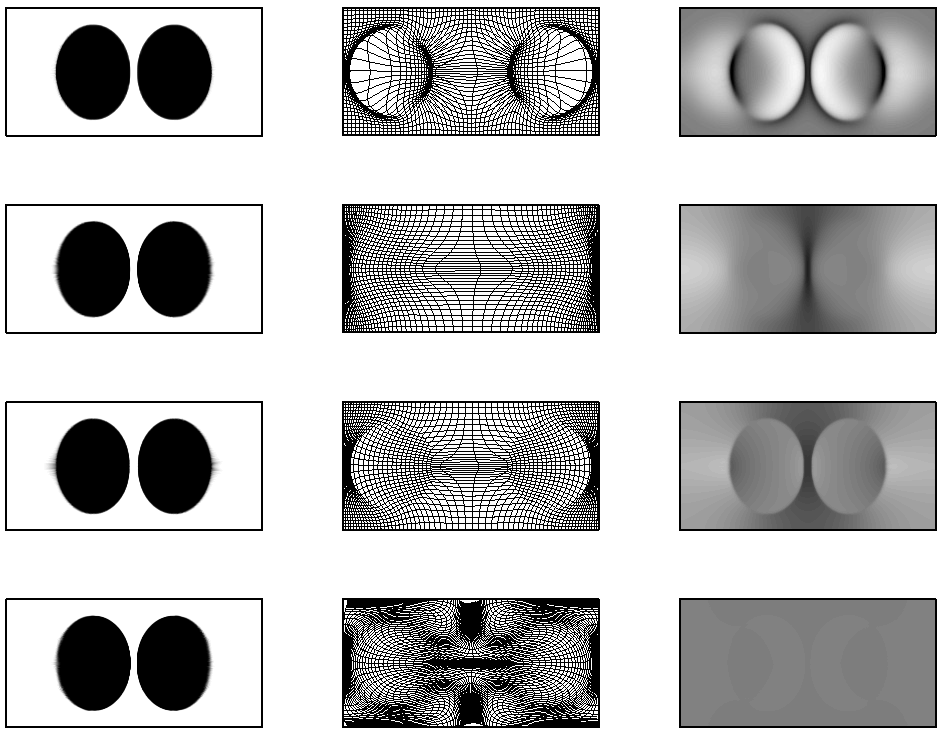
\includegraphics[width=\textwidth]{figure2Dii}
%\end{columns}
%\end{frame}



%\begin{frame}
%\frametitle{Change of Variables}
%When we warp images, we should usually account for expansion/contraction via a change of variables.
%\begin{eqnarray*}
%\int_{{\bf x} \in \varphi(\Omega)} f({\bf x}) d{\bf x} = \int_{{\bf x} \in \Omega} f(\varphi({\bf x})) \det |({\bf D}\varphi)({\bf x})| d{\bf x}
%\end{eqnarray*}
%where $({\bf D}\varphi)({\bf x})$ means the Jacobian of $\varphi$ at ${\bf x}$.
%\end{frame}

%%%%%%%%%%%%%%%%%%%%%%%%%%%%%%%%%%%%%%%%%%%%%%%%%%%%%%%%%%%%%%%

%\begin{frame}
%\frametitle{LDDMM}
%Estimating a series of velocity fields looks like it involves estimating a lot of parameters, but this is not actually the case.
%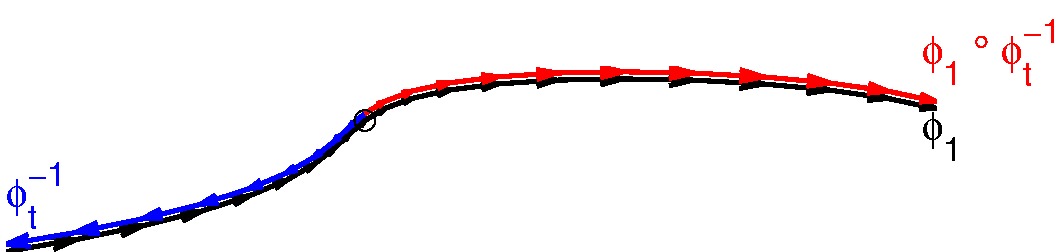
\includegraphics[width=\textwidth]{trajectory}

%The matching term of the objective function is:
%\begin{eqnarray*}
%\frac{1}{2\sigma^2} \int_{x\in\Omega} ( f \circ {\bf x} - \mu \circ {\boldsymbol\varphi}_{1}^{-1} \circ {\bf x})^2 d{\bf x}
%\end{eqnarray*}

%This may be re-written (including a change of variables) as:
%\begin{eqnarray*}
%\frac{1}{2\sigma^2} \int_{x\in\Omega} \det |{\bf D}( {\boldsymbol\varphi}_{1} \circ {\boldsymbol\varphi}_{t}^{-1}) \circ {\bf x} | ( f \circ {\boldsymbol\varphi}_1 \circ {\boldsymbol\varphi}_{t}^{-1} \circ {\bf x} - \mu \circ {\boldsymbol\varphi}_{t}^{-1} \circ {\bf x})^2 d{\bf x}
%\end{eqnarray*}
%This allows the derivatives of the matching term to be computed at any time point.
%\end{frame}

